\documentclass[12pt]{article}

%\usepackage{fancyhdr}   % header y footer

% Márgenes 
\topmargin=-0.45in      %
\evensidemargin=0in     %
\oddsidemargin=0in      %
\textwidth=6.5in        %
\textheight=9.0in       %
\headsep=0.25in         %

% Acentos en castellano
% \usepackage[latin1]{inputenc} % iso-8889-1
\usepackage[utf8]{inputenc} % utf-8

\usepackage{graphicx}    % imagenes
% Soporte para hyperlinks.

\usepackage{hyperref}

\usepackage[T1]{fontenc}
\usepackage{mathtools}

% Temporal para las anotaciones de cosas a rellenar
\usepackage{color}
\usepackage{listings}             % Para poner código
\usepackage{natbib}

\usepackage{color}
\usepackage{caption}
\usepackage{subcaption}


\definecolor{mygreen}{rgb}{0,0.6,0}
\definecolor{mygray}{rgb}{0.5,0.5,0.5}
\definecolor{mymauve}{rgb}{0.58,0,0.82}
\definecolor{light-gray}{gray}{0.95}

\lstset{ %
  backgroundcolor=\color{light-gray},   % choose the background color; you must add \usepackage{color} or \usepackage{xcolor}
  basicstyle=\footnotesize,        % the size of the fonts that are used for the code
  breakatwhitespace=false,         % sets if automatic breaks should only happen at whitespace
  breaklines=true,                 % sets automatic line breaking
  captionpos=b,                    % sets the caption-position to bottom
  commentstyle=\color{mygreen},    % comment style
  deletekeywords={...},            % if you want to delete keywords from the given language
  escapeinside={\%*}{*)},          % if you want to add LaTeX within your code
  extendedchars=true,              % lets you use non-ASCII characters; for 8-bits encodings only, does not work with UTF-8
  %frame=single,                    % adds a frame around the code
  keepspaces=true,                 % keeps spaces in text, useful for keeping indentation of code (possibly needs columns=flexible)
  keywordstyle=\color{blue},       % keyword style
  language=C,                 % the language of the code
  morekeywords={*, ..., For, If, :=>, <=, free, function, While},            % if you want to add more keywords to the set
  numbers=left,                    % where to put the line-numbers; possible values are (none, left, right)
  numbersep=5pt,                   % how far the line-numbers are from the code
  numberstyle=\tiny\color{mygray}, % the style that is used for the line-numbers
  rulecolor=\color{black},         % if not set, the frame-color may be changed on line-breaks within not-black text (e.g. comments (green here))
  showspaces=false,                % show spaces everywhere adding particular underscores; it overrides 'showstringspaces'
  showstringspaces=false,          % underline spaces within strings only
  showtabs=false,                  % show tabs within strings adding particular underscores
  stepnumber=1,                    % the step between two line-numbers. If it's 1, each line will be numbered
  stringstyle=\color{mymauve},     % string literal style
  tabsize=2,                       % sets default tabsize to 2 spaces
  title=\lstname                   % show the filename of files included with \lstinputlisting; also try caption instead of title
}




% Nombres de contenido generado automáticamente (como tabla de contenidos)
% en español. Para poder usarlo:
% sudo apt-get install texlive-lang-spanish
%
% Comentado mientras no sea necesario para nada mas; podemos cambiar
% el nombre de la tabla de contenidos a mano, puesto que este paquete
% parece que fuerza los números de página románicos a ser en mayúscula.
\usepackage[spanish]{babel}

\begin{document}

\title{
     {\bf Neurocomputación} \\
     Práctica 3:\\ {\bf Aplicaciones del Perceptrón Multicapa}.\\
}
\author{
     Daniel Gutiérrez Navío \\
     Matías Bender \\
     \textit{Grupo 2461}
}
\date{\today}

\maketitle

% necesario quitar el estilo de página después de \maketitle para quitar el
% primer numero de pagina, porque \maketitle hace \pagestyle{plain}
\thispagestyle{empty}
\newpage

% numeración romana para las primeras páginas
\pagenumbering{roman}

%\renewcommand*\contentsname{Índice}
\tableofcontents
%\listoffigures
\newpage

\bibliographystyle{alpha}
%\bibliography{sample}

% numeración arábica para el resto del documento
\setcounter{page}{1}
\pagenumbering{arabic}

% indentacion primera linea de parrafo
\setlength{\parindent}{0pt}

% distancia entre parrafos
\setlength{\parskip}{8pt}

% Parte 1: Manual de uso (si se necesita)
%%%%%%%%%%%%%%%%%%%%%%%%%%%%%%%%%%%%%%%%%%%%%%%%%%%%%%%%%%%%%%%%%%%%%%%%%%%
%el section del manual se pone como está comentado aquí, para que salga sin número pero en el índice
%\phantomsection
%\addcontentsline{toc}{section}{Manual de uso}
%\section*{Manual de uso}

\newpage

\section{Autoenconder}

Un autoencoder es una red neuronal usada para aprender y buscar codificaciones eficientes. Sus aplicaciones más importantes son la eliminación de ruido y distorsiones en la entrada, y la compresión de datos. El objetivo de este es aprender a comprimir, desde un conjunto de datos, una codificación. Para ello se utilizan redes cuya salida es igual a la entrada. Se busca que la red capture la estructura interna del problema. En la siguiente sección analizaremos el problema de compresión de codificaciones utilizando esta idea.

Buscaremos codificar una conjunto de imagenes de N pixeles X N pixeles con dos tonos, compuestas solamente por un máximo de dos lineas verticales y/o horizontales.

  \begin{figure}[!ht]
    \centering
    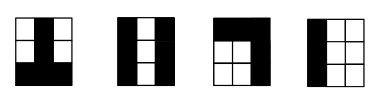
\includegraphics[width=10cm]{ejemplo}
  \end{figure}

Para ello utilizaremos un Perceptron Multicapa al que entrenaremos con todas las posibles imagenes, poniendo como objetivo que las aprenda en su totalidad. El parámetro a estimar es la cantidad de neuronas en la capa oculta necesarias para que el problema sea resuelto. Si obtenemos un número menor de neuronas en esta capa que en la de entrada, entonces podremos codificar o decoficar estas imagenes utilizando para eso las activaciones de la capa oculta, que serán menos que los datos de entrada.

\subsection{Im\'agenes de 3x3}

Considerando todas las imagenes de 3 pixeles x 3 pixeles que cumplen las condiciones de este problema, la cantidad de neuronas necesarias, en la capa oculta, para aprender el problema es 5. Dado que no importa demasiado cu\'antas iteraciones tarda el algoritmo en aprender, si no que aprenda correctamente, el factor de aprendizaje puede ser tomado como un número chico, en este caso $0.1$.

En los siguientes gráficos se puede observar como evoluciona tanto el Error Cuadrático Medio ,medido en la cantidad de pixeles equivocados, como el porcentaje de estos pixeles sobre el total hasta converger totalmente en 5 neuronas.

\begin{figure}[!ht]
\centering
    \begin{subfigure}[b]{0.5\textwidth}            
            \centering
            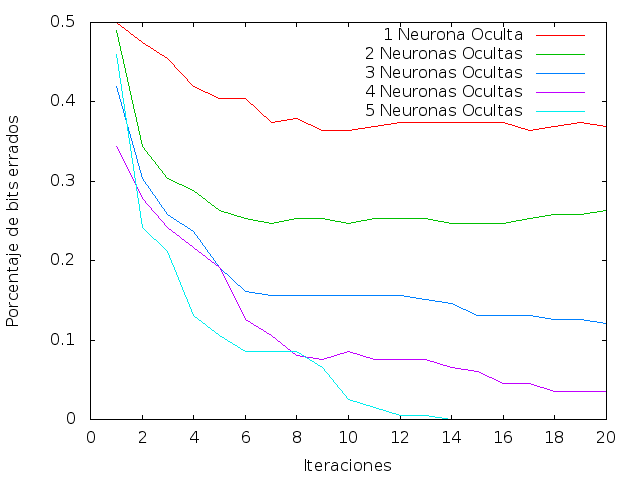
\includegraphics[width=\textwidth]{graficosde3neuronas/imagenDistancia}
            \caption{Porcentaje de p\'ixeles equivocados seg\'un \'epoca}
            \label{fig:dist_3}
    \end{subfigure}%
     %add desired spacing between images, e. g. ~, \quad, \qquad etc.
      %(or a blank line to force the subfigure onto a new line)
    \begin{subfigure}[b]{0.5\textwidth}
            \centering
            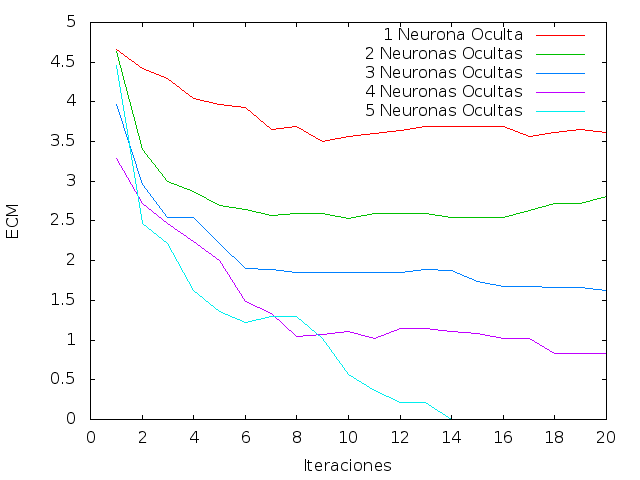
\includegraphics[width=\textwidth]{graficosde3neuronas/imagenECM}
            \caption{ECM de los p\'ixeles equivocados}
            \label{fig:ecm_3}
    \end{subfigure}
    \caption{Entrenamiento con distinta cantidad de neuronas en la capa oculta}
  \label{fig:graph3}
\end{figure}

Es interesante observar que con 4 neuronas la red aprende casi todos los patrones. El único patrón en el que siempre falla con esa arquitectura es en la imagen sin lineas. Más adelante reflexionaremos sobre ello.

De esta manera, con solo 5 números podemos caracterizar el patrón del cual estamos hablando. Sin embargo, hay que tener mucho cuidado si se está pensando en una codificación real. Los números de los cuales se hablan son números de punto flotante, o sea que ocupan 32b cada uno (el doble si son de doble presición). Si la codificación original toma un Integer (32b) para almacenar cada pixel, el beneficio de la nueva codificación es de $180\%$ la original. Sin embargo, podrían llegar a codificarse 32 pixeles en un solo Integer, por lo que en este caso, la codificación del autoencoder sería $20\%$ de la original, o sea gastaría $5$ veces su cantidad de memoria. 

Vale la pena tomarse un tiempo (quizás no tan corto) para analizar qué está ocurriendo en la red neuronal entrenada una vez que aprende perfectamente todos los patrones. Para lograr dicho objetivo decidimos observar cuál es la activación de cada neurona en la capa oculta según cada ejemplo de entrada y con eso agruparlas según clases que permitan observar lo que está ocurriendo. El primer acercamiento consistió en tomar dos clases distintas, la de las activaciones mayores a cero y las de las menores. Sin embargo, no era poder identificar unívocamente a cada elemento conociendo simplemente la clase a la que pertence según cada neurona oculta. O sea, había dos entradas que pertenencían a las mismas clases en cada neurona, por lo que no se podía ver qué era lo que las diferenciaba. El segundo acercamiento consistió en cuatro clases según la salida de cada neurona, las menores a $-0.5$, las negativas mayores a $-0.5$, las positivas menores a $0.5$ y las positivas mayores a $0.5$. A continuación se muestra el resultado de esta clasificación.

\begin{center}
   \begin{tabular}{| c | c | c | c | c |}
     \hline
      & $-1<n<-0.5$ & $-0.5<n<0$ & $0<n<0.5$ & $0.5<n<1$ \\ \hline
     Neurona 1 &
     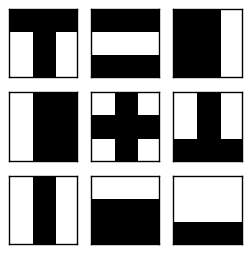
\includegraphics[width=2cm]{graficosde3neuronas/atributo0Clase0} &
     
\includegraphics[width=2cm]{graficosde3neuronas/atributo0Clase1} &
     
\includegraphics[width=2cm]{graficosde3neuronas/atributo0Clase2} &
     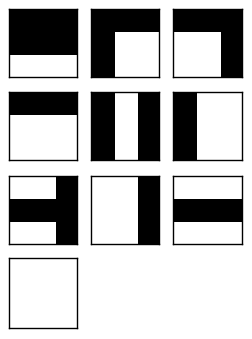
\includegraphics[width=2cm]{graficosde3neuronas/atributo0Clase3} \\ \hline
     Neurona 2 &
     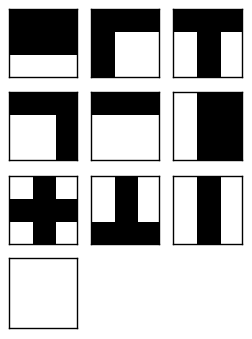
\includegraphics[width=2cm]{graficosde3neuronas/atributo1Clase0} &
     
\includegraphics[width=2cm]{graficosde3neuronas/atributo1Clase1} &
     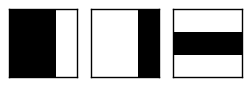
\includegraphics[width=2cm]{graficosde3neuronas/atributo1Clase2} &
     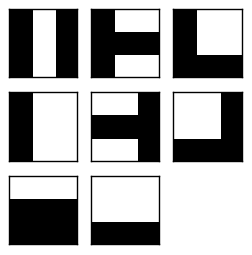
\includegraphics[width=2cm]{graficosde3neuronas/atributo1Clase3} \\ \hline
     Neurona 3 &
     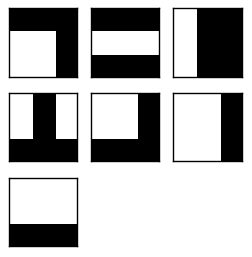
\includegraphics[width=2cm]{graficosde3neuronas/atributo2Clase0} &
     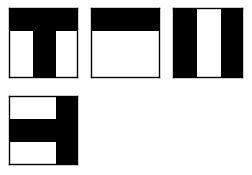
\includegraphics[width=2cm]{graficosde3neuronas/atributo2Clase1} &
     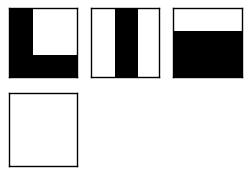
\includegraphics[width=2cm]{graficosde3neuronas/atributo2Clase2} &
     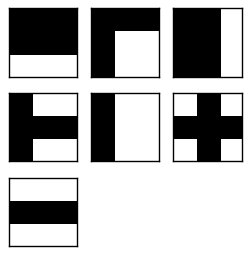
\includegraphics[width=2cm]{graficosde3neuronas/atributo2Clase3} \\ \hline
     Neurona 4 &
     
\includegraphics[width=2cm]{graficosde3neuronas/atributo3Clase0} &
     
\includegraphics[width=2cm]{graficosde3neuronas/atributo3Clase1} &
     
\includegraphics[width=2cm]{graficosde3neuronas/atributo3Clase2} &
     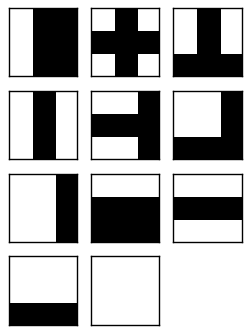
\includegraphics[width=2cm]{graficosde3neuronas/atributo3Clase3} \\ \hline
     Neurona 5 &
     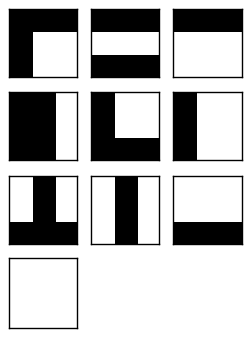
\includegraphics[width=2cm]{graficosde3neuronas/atributo4Clase0} &
     
\includegraphics[width=2cm]{graficosde3neuronas/atributo4Clase1} &
     
\includegraphics[width=2cm]{graficosde3neuronas/atributo4Clase2} &
     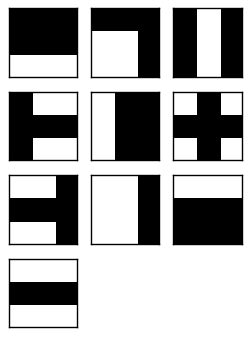
\includegraphics[width=2cm]{graficosde3neuronas/atributo4Clase3} \\ \hline
   \end{tabular}
 \end{center}

En estos gráficos podemos notar diferentes cosas. La primera es que la mayoría de las entradas causan que las neuronas de la capa oculta tomen valores de salida distantes entre ella, o sea, las neuronas clasifican con más seguridad dado que el patrón que detectan los detectan con bastante seguridad, dado que toman valores de salida, en modulo, cercanos a $1$. Esta es la causa fundamental por la que la codificación es eficiente, dado que se encuentran patrones determinantes para cada imagen.

Por otro lado, podemos notar como los complementos de las imagenes se encuentran siempre en categorías enfrentadas. Esto ocurre por la codificación que se tiene de los parámetros donde los blancos se representan con $-0.9$ y los negros con $0.9$, por lo que invertir los colores es multiplicar por $-1$ las entradas.

Yendo más al detalle, podemos observar como la Neurona 1 asigna valores más bajos a todas las entradas que tienen una linea vertical en el centro. A su vez, asigna valores más grandes a todas las que tienen una linea vertical a la derecha en mayor medida y a izquierda en menor, salvo que caigan en el caso anterior. La Neurona 2 asigna valores más bajos a quien tenga una linea horizontal arriba, y más altos a quien la tenga en el centro. La Neurona 3 asigna valores más bajos a las imagenes con mayor concentración de pixeles arriba a la izquierda, mientras que más altos a quienes se concentran más a la derecha, aquí se puede ver como la clasificación no es tan exacta teniendo mayor grado de impresición (varios valores menores en módulo a $-0.5$). La Neurona 4, asigna valor más bajo a las imagenes con más de una linea y mayor a las que tienen menos lineas. Por último, la Neurona 5 se comporta como la neurona 3, pero pondera distinto según las lineas horizontales. 

\subsection{Imágenes más grandes}

Se analizaron casos donde las imagenes constaban de más píxeles, pero dados los tiempos de procesamiento y la busqueda de los valores óptimos se analizará el caso concreto de 5 píxeles X 5 píxeles. Aquí podemos encontrar que se necesitan 9 neuronas en la capa oculta para aprender perfectamente el problema, y se vuelve a apreciar el hecho de que con 8 neuronas no aprende el caso de la imagen vacía. Creemos que la razón de esto se haya en el hecho de que hay más pixeles en blanco que en negro, por lo que el peso de un pixel en negro es ponderado más que un pixel en blanco dado que transmite más información. Luego, la imagen vacia, o toda en blanco, tiene poca información que hace que la red esté indecisa y falle. Esto es esperable dado que siempre es mejor entrenar a la red neuronal con casos parejos entre los valores de la entrada, misma cantidad de negros y de blancos entre el total de todas las imagenes.

\begin{figure}[!ht]
\centering
    \begin{subfigure}[b]{0.5\textwidth}            
            \centering
            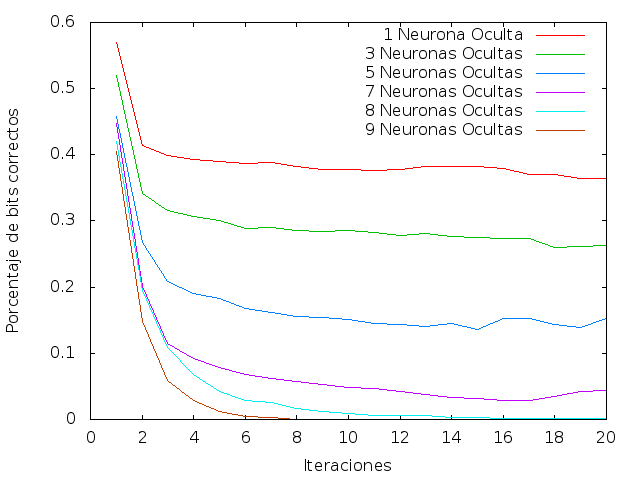
\includegraphics[width=\textwidth]{graficosde5neuronas/imagenDistancia}
            \caption{Porcentaje de p\'ixeles equivocados seg\'un \'epoca}
            \label{fig:dist_5}
    \end{subfigure}%
     %add desired spacing between images, e. g. ~, \quad, \qquad etc.
      %(or a blank line to force the subfigure onto a new line)
    \begin{subfigure}[b]{0.5\textwidth}
            \centering
            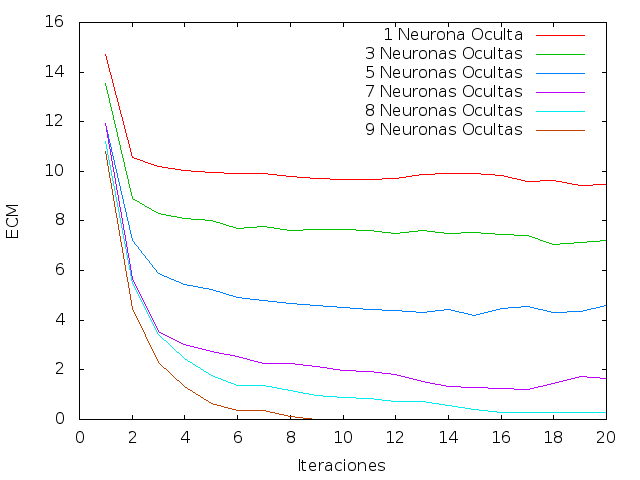
\includegraphics[width=\textwidth]{graficosde5neuronas/imagenECM}
            \caption{ECM de los p\'ixeles equivocados}
            \label{fig:ecm_5}
    \end{subfigure}
    \caption{Entrenamiento con distinta cantidad de neuronas en la capa oculta}
  \label{fig:graph5}
\end{figure}

Aquí nuevamente se intentó, esta vez con menos éxito, analizar el tipo de clasificación que hace cada neurona. Dada la complejidad de esta tarea por la cantidad de imagenes posibles, solo haremos dos pequeñas menciones. Aquí nuevamente se observa que el clustering con dos clases falla al determinar unívocamente cada entrada, sin embargo el clustering de 4 categorías funciona perfectamente. Es importante comentar que nuevamente los valores de salida se volcaron hacía los extremos, módulo mayor a $0.5$, lo que refuerza las bondades de usar estos autoencoders. Por lo dicho antes, solo mostraremos lo que ocurre con solo una neurona de la capa oculta. Como se puede ver en la imagen, los valores más bajos correspoden a imagenes con más concentración de pixeles negros en el centro. Los más altos, los que menos píxeles en la mitad tienen.

\begin{center}
   \begin{tabular}{| c | c | c | c |}
     \hline
     %Atributo 1 
     $-1<n<-0.5$ & $-0.5<n<0$ & $0<n<0.5$ & $0.5<n<1$ \\ \hline
     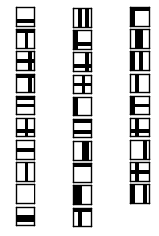
\includegraphics[width=4cm]{graficosde5neuronas/atributo1Clase0} &
     
\includegraphics[width=2.5cm]{graficosde5neuronas/atributo1Clase1} &
     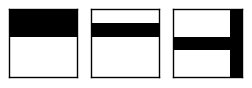
\includegraphics[width=2.5cm]{graficosde5neuronas/atributo1Clase2} &
     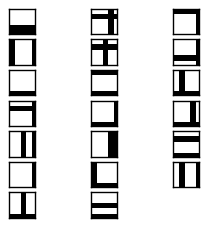
\includegraphics[width=4cm]{graficosde5neuronas/atributo1Clase3} \\ \hline
   \end{tabular}
 \end{center}

\newpage

\section{Predicción tendencia en series temporales}

Un problema típico para las redes neuronales es la predicción de series temporales. Mediante información sobre la tendencia en puntos anteriores, con una red neuronal, es posible predecir que valores o características tendrá una serie temporal en los siguientes puntos.

En esta parte de la práctica, deberemos realizar un sistema basado en un perceptrón multicapa que sea capaz de predecir la tendencia, ascendente o descendente, de los siguientes puntos de una serie temporal basándose en datos pasados de la serie.

Realizaremos una función, adapta-serie-temporal, que nos traducirá, dado un argumento llamado np, la serie temporal en un fichero que nuestra red pueda interpretar. Dado ese fichero, realizaremos predicciones sobre la serie temporal.

Ahora realizaremos un estudio del funcionamiento de las predicciones con distintos parámetros (valores de np, neuronas ocultas, y porcentaje de la serie en training), para dos series diferentes: una primera serie sinusoidal, y otra caótica.

\subsection{Predicción sobre serie sinusoidal}

En esta sección estudiaremos el comportamiento de las predicciónes sobre esta serie. La serie en concreto, es la siguiente:
\begin{center}
	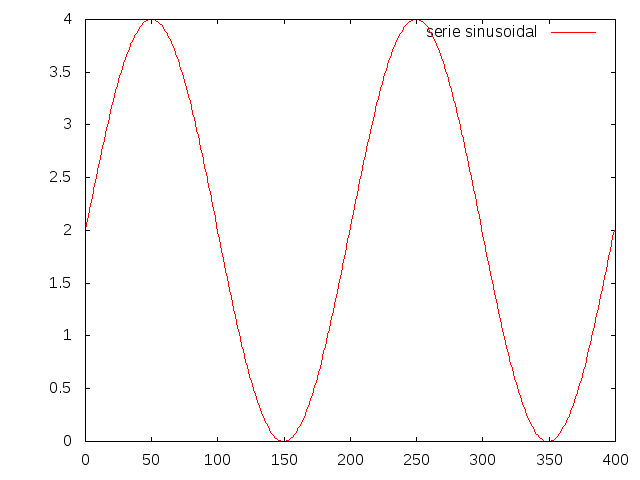
\includegraphics[width=8cm]{serie_sinusoidal}
\end{center}

Como podemos apreciar, es una serie sinusoidal, un seno en concreto. Al realizar un comportamiento monótono creciente, hasta llegar a un punto de monotonía descendente, importará en un principio el \% que introduzcamos en training. Si metemos todo el comportamiento, podrá en un principio predecir todo facilmente, mientras que si metemos una sola parte, tendrá problemas.

En concreto, dados sus 400 valores, con 100 no llega a capturar todo su comportamiento. Sin embargo, mostraremos que, con una cantidad suficiente de puntos previos, np, podrá llegar a predecir con bastante exactitud el comportamiento. Esto, es debido a que llega a predecir, que si una parte de sus valores es descendente, y otra parte ascendente, tiene que cambiar el valor de la predicción. Esto sólo será posible con valores de np elevados, lo cuál mostraremos a continuación.

Primero, realizaremos un estudio de, según cuántas neuronas, con np = 1, 2 y 5, su porcentaje de error y ECM, para ver el tamaño en neuronas adecuado para la serie. Probaremos tamaño de capa oculta de 2, 3 y 5.

Primero observemos el comportamiento con 100 elementos de entrenamiento.

Empezaremos a mirar np=1. Con este tamaño, no debe ser posible con 2 neuronas, probaremos con 3, 4 y 5 para obtener mayor información posible. Observemos los gráficos de error y ecm:

\begin{center}
   \begin{tabular}{ c  c }
     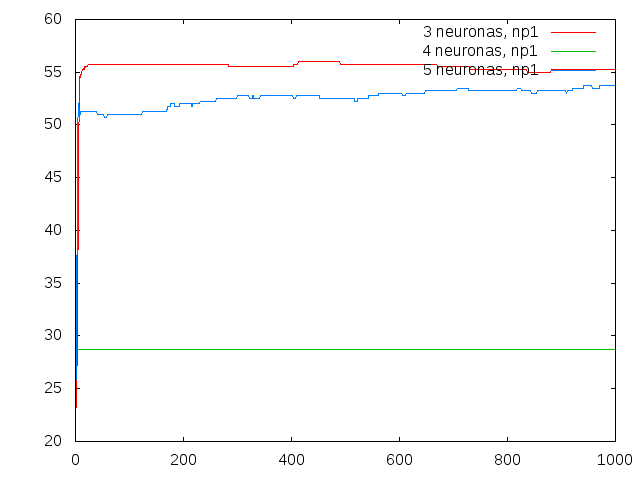
\includegraphics[width=6cm]{graficosparte2a/error_train_np1_25} &
     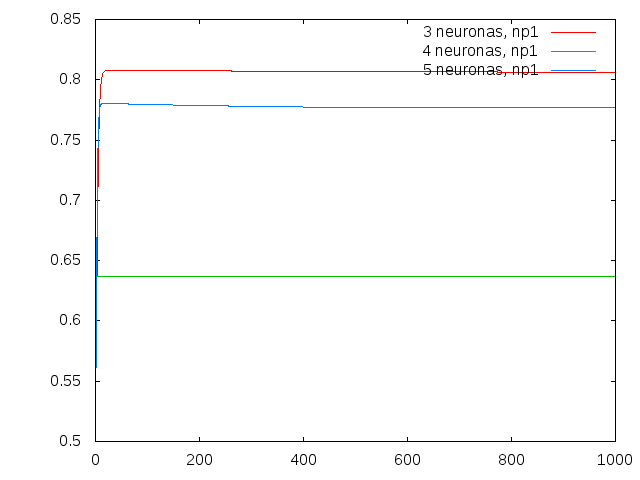
\includegraphics[width=6cm]{graficosparte2a/ecm_train_np1_25}\\ 
   \end{tabular}
 \end{center}
 
Podemos ver, que el error y el ECM son constantes, por lo que no hay entrenamiento, además de ser altos.

En el test, estos valores dan un resultado constante de 50.5, siendo esto un resultado pésimo, dando de conclusión que np1 no es un tamaño adeucado. No es posible la predicción con un solo valor anterior.

Ahora, veamos con np=2:

\begin{center}
   \begin{tabular}{ c  c }
     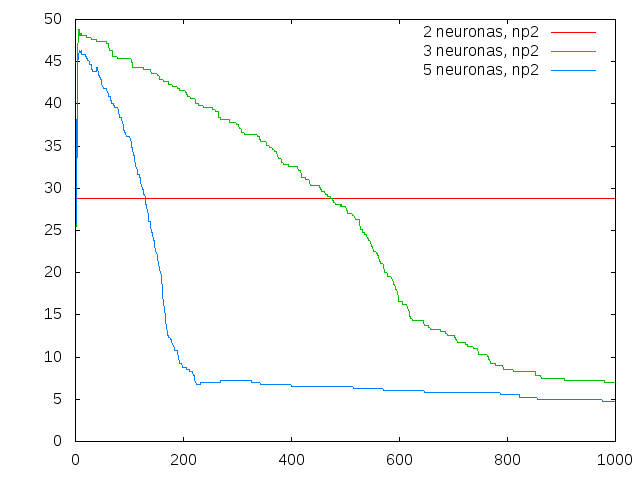
\includegraphics[width=6cm]{graficosparte2a/error_train_np2_25} &
     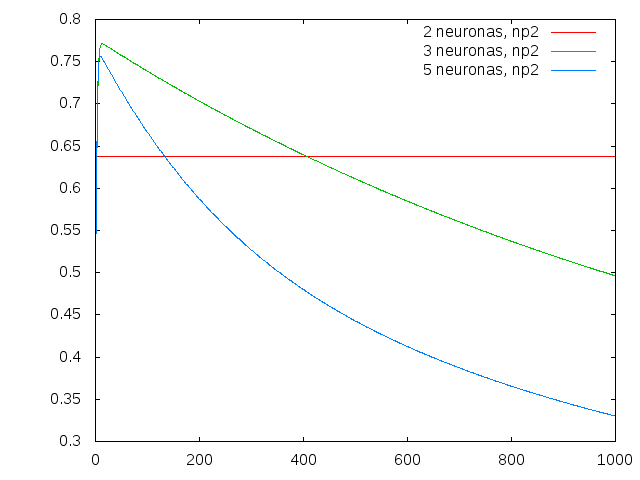
\includegraphics[width=6cm]{graficosparte2a/ecm_train_np2_25}\\ 
   \end{tabular}
 \end{center}
 
 Podemos ver que ahora si existe cierto entrenamiento, dado que la gráfica de ECM en 3 y 5 neuronas, tiende a descender, siginifica que va mejorando.
 
 Llega a un mínimo de error en el caso de 5 neuronas sobre la época 200, mientras que llega en el caso de 3 sobre la 800-900.
 
 Esto sugiere un mejor comportamiento en este problema con 5 neuronas. Iremos a partir de ahora fijandonos de manera especial en el caso de 5 neuronas.
 
 Ahora veamos el error en el test:
 
\begin{center}
	\begin{tabular}{| c | c |}
		\hline
		Neuronas & Error \\ \hline
		2 & 46.7337\% \\ \hline
		3 & 59.799\% \\ \hline
		5 & 79.8995\% \\ \hline
	\end{tabular}
\end{center}

Se puede apreciar que el caso con 5 neuronas, es bastante más preciso que el resto. Debido a la mayor capacidad me memoria interna, muy probablemente, al tener mas pesos.

Veamos el caso de np=5, esta vez solo con 3 y 5 neuronas, dado que 2 se ha demostrado muy inferior, de hecho, sin capacidad para aprender:

\begin{center}
   \begin{tabular}{ c  c }
     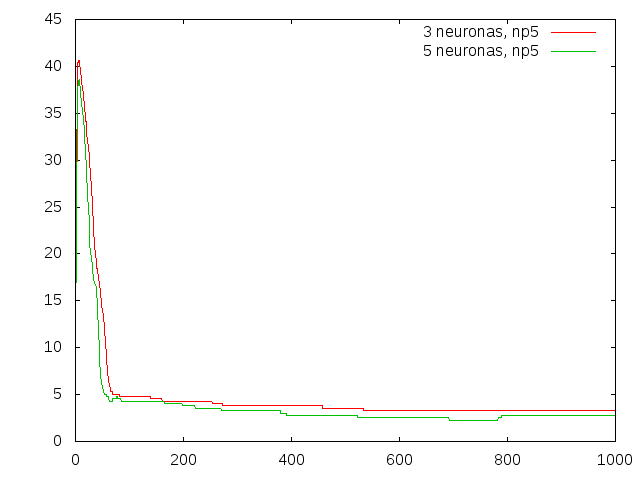
\includegraphics[width=6cm]{graficosparte2a/error_train_np5_25} &
     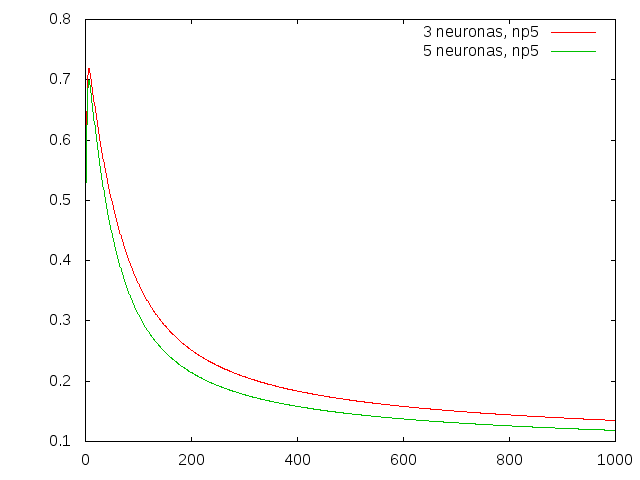
\includegraphics[width=6cm]{graficosparte2a/ecm_train_np5_25}\\ 
   \end{tabular}
 \end{center}

Aquí podemos ver ambos casos con muy buen resultado en entrenamiento, lo que significa que ya aprende correctamente,en ambos. Además, ambas redes aprenden al mismo tiempo prácticamente.

Observemos el resultado del test:

\begin{center}
	\begin{tabular}{| c | c |}
		\hline
		Neuronas & Error \\ \hline
		3 & 93.9394\% \\ \hline
		5 & 96.9697\% \\ \hline
	\end{tabular}
\end{center}

Viendo esto, podemos afirmar que el tamaño de la capa oculta óptimo, empiricamente hablando, es de 5, y np óptimo, de 5 también.

Ahora observemos el comportamiento con 200 elementos en entrenamiento:

\begin{center}
   \begin{tabular}{ c  c }
     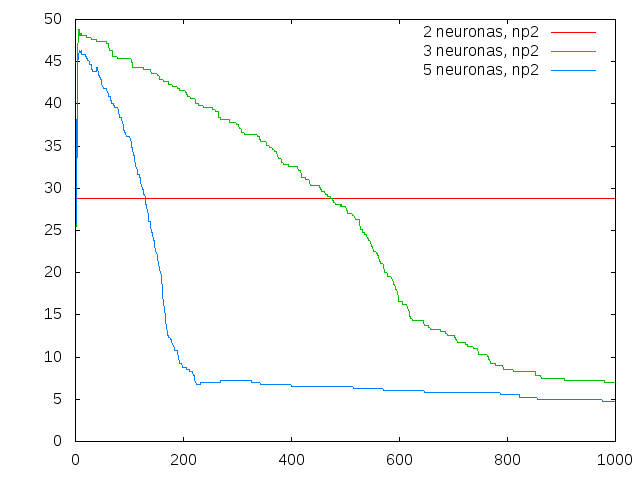
\includegraphics[width=6cm]{graficosparte2a/error_train_np2} &
     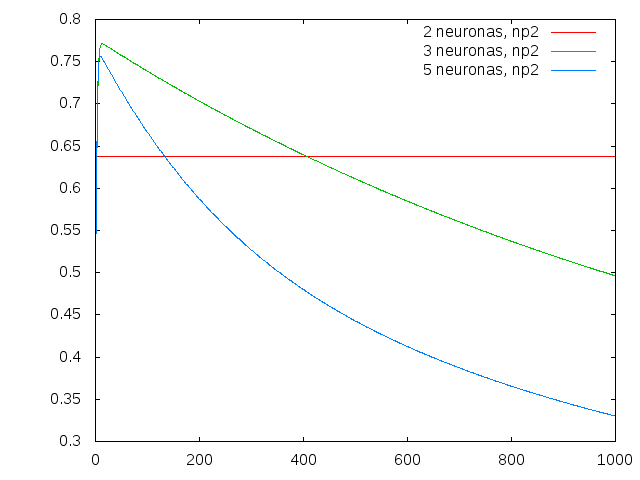
\includegraphics[width=6cm]{graficosparte2a/ecm_train_np2}\\ 
   \end{tabular}
 \end{center}

Podemos, en las gráficas que vemos arriba, observar el comportamiento de el error y error cuadrático medio, en la etapa de entrenamiento, para 2, 3 y 5 neuronas, durante 1000 epocas de entrenamiento, con np = 2.

Podemos observar que en el caso de 2 neuronas, tiene un entrenamiento plano, es decir, no llega a aprender. Con 3 y 5 neuronas, se puede apreciar que aprende, llegando a convergencia en errores con 5 neuronas en la epoca 200, y con 3 sobre la epoca 900.

Observemos ahora el error que resulta de aplicar al test de las otras 200 instancias no usadas en entrenamiento:

\begin{center}
	\begin{tabular}{| c | c |}
		\hline
		Neuronas & Error \\ \hline
		2 & 46.733\% \\ \hline
		3 & 59.799\% \\ \hline
		5 & 78.8995\% \\ \hline
	\end{tabular}
\end{center}

Como podemos ver, en ninguno de los casos llega a un número de errores similar al test. Esto es, pese a tener la mitad, debido a que no tiene suficientes elementos en la serie.

Realizaremos ahora las mismas pruebas con np=3

\begin{center}
   \begin{tabular}{ c  c }
     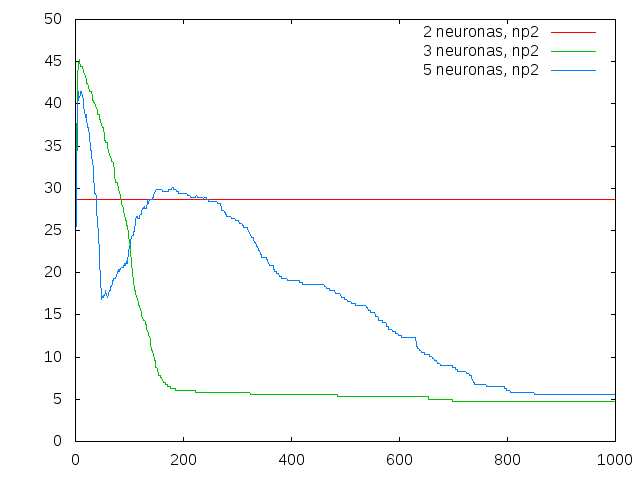
\includegraphics[width=6cm]{graficosparte2a/error_train_np3} &
     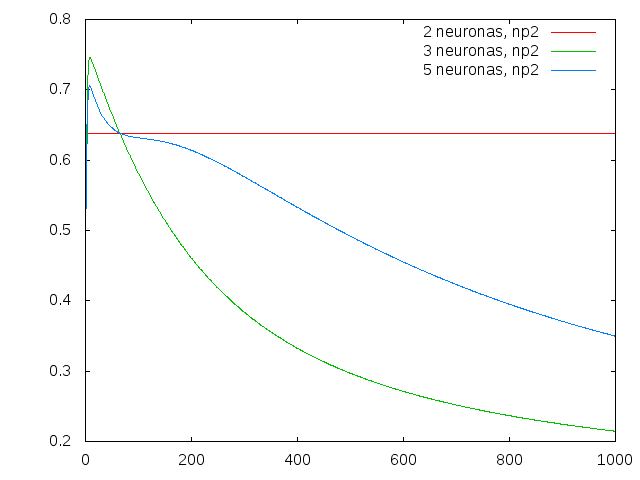
\includegraphics[width=6cm]{graficosparte2a/ecm_train_np3}\\ 
   \end{tabular}
 \end{center}
 

En este caso, el tamaño óptimo en número de neuronas es 3, dado que alcanza un valor mejor y antes, en error y ecm. El caso de 2 neuronas, sigue siendo totalmente plano, sin llegar a aprender en ningún momento.

La convergencia se llega en el caso de 3 neuronas, en la época 180, y de 5 en la época 800.

Estos casos de enetrenamiento son mejores que los de np=2. Sin embargo, observemos los resultados del test:

\begin{center}
	\begin{tabular}{| c | c |}
		\hline
		Neuronas & Error \\ \hline
		2 & 42.7237\% \\ \hline
		3 & 85.9296\% \\ \hline
		5 & 79.8995\% \\ \hline
	\end{tabular}
\end{center}

El caso de 5 neuronas y 2 no ha cambiado. Sin embargo, existe una mejoría clara en el caso de 3 neuronas.

Observemos ahora el comportamiento con np=5. Para esta vez, ya que hemos visto el pésimo comportamiento de 2 neuronas, descartaremos este caso:

\begin{center}
   \begin{tabular}{ c  c }
     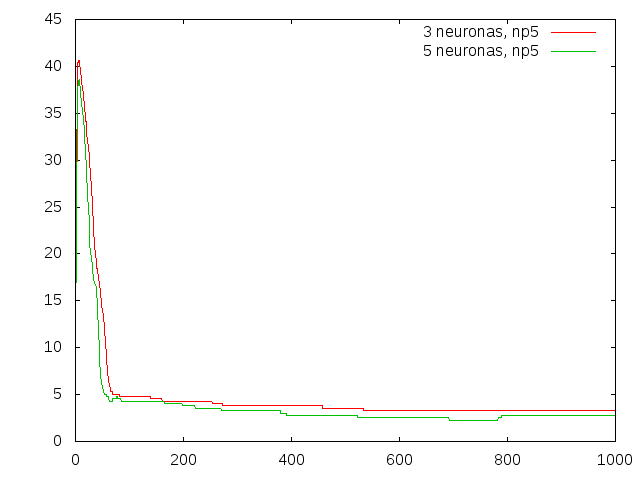
\includegraphics[width=6cm]{graficosparte2a/error_train_np5} &
     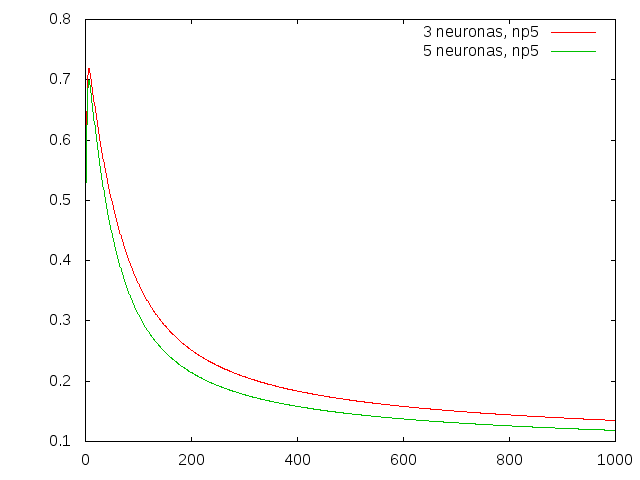
\includegraphics[width=6cm]{graficosparte2a/ecm_train_np5}\\ 
   \end{tabular}
 \end{center}

Ahora vemos, que ambas se comportan de manera similar, llegando a una convergencia prácticamente en la época 80.

Para poder observar mejor cuál es el número óptimo, deberemos ver ahora el caso de test:

\begin{center}
	\begin{tabular}{| c | c |}
		\hline
		Neuronas & Error \\ \hline
		3 & 93.9394\% \\ \hline
		5 & 96.9697\% \\ \hline
	\end{tabular}
\end{center}

Aquí,con np=5, podemos observar que el perceptrón ya es capaz de conseguir predecir la monotonía futura de la función.

Comparando ambos casos, usando 100 y 200 para entrenamiento, hemos visto que con un número grande de neuronas aprende igual, y consigue un resultado identico en test.

Esto es debido a que lo que el perceptrón analiza, no es la forma que ve, sino la monotonía, y sabe que para cambiar su monotonía, debe haber un cambio en la monotonía de la serie.
\newpage
\subsection{Serie Caótica}

En este apartado, realizaremos un análisis similar al anterior, sobre una serie caótica dada. La serie es la siguiente:

\begin{center}
	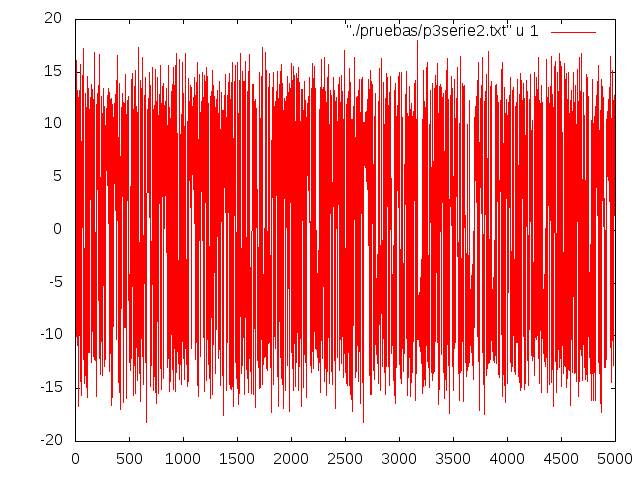
\includegraphics[width=10cm]{serie_caotica}
\end{center}

Podemos ver que no tiene un patrón fijo de subidas y bajadas. Sus valores tienen una gran variabilidad. Sin embargo, pese a que predecir esta red debe ser dificil, predecir su monotonía, no es complejo. Además, por la variabilidad de valores, el resultado usando partición del 25\% y del 50\%, debe ser similar. Por ello, haremos la predicción usando partición del 25\%. Al final demostraremos con un ejemplo esto.

Probaremos usando 5 neuronas, dado que en la anterior sección vimos que era el mejor caso, para ver cuál es el mejor np para este problema (numero de muestras anteriores). Una vez hallado el número de muestras idóneo, probaremos distinto tamaño de capa oculta.

\begin{center}
   \begin{tabular}{ c  c }
     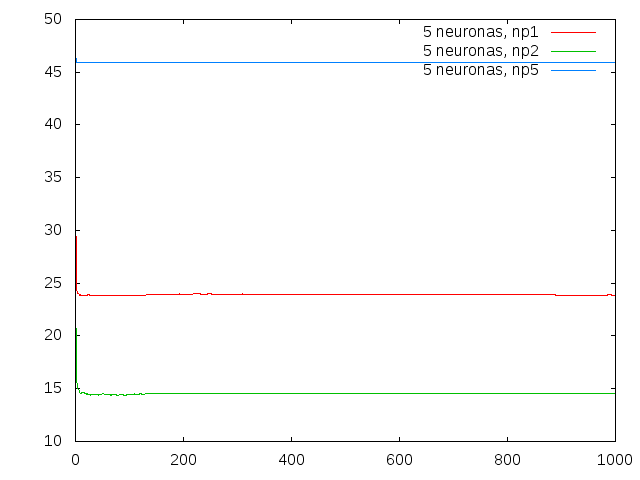
\includegraphics[width=6cm]{graficosparte2a/error_train_caotic_5n} &
     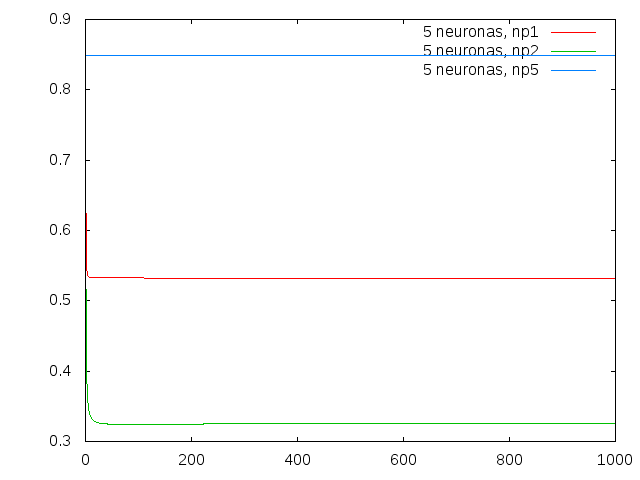
\includegraphics[width=6cm]{graficosparte2a/ecm_train_caotic_5n}\\ 
   \end{tabular}
 \end{center}

Se puede ver que alcanza muy pronto a una convergencia, por lo que ampliaré a sólo las 40 primeras épocas.

\begin{center}
   \begin{tabular}{ c  c }
     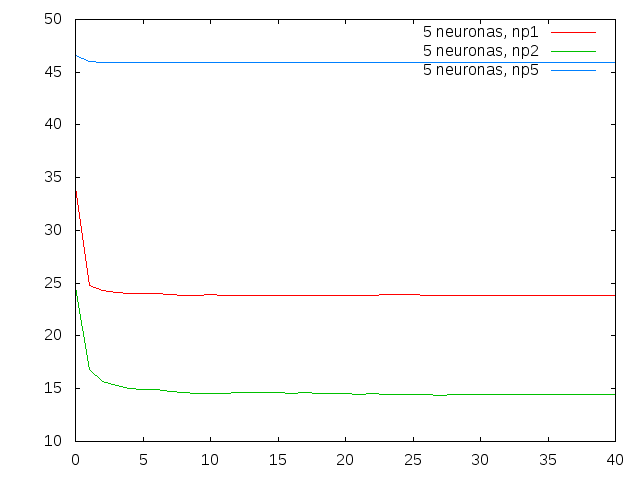
\includegraphics[width=6cm]{graficosparte2a/error_train_caotic_5n_200} &
     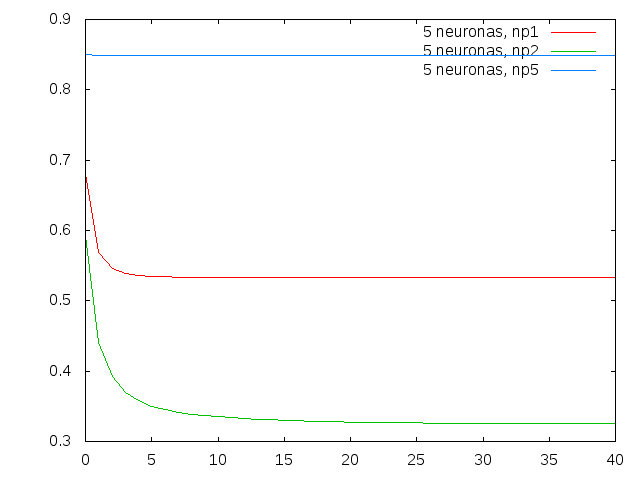
\includegraphics[width=6cm]{graficosparte2a/ecm_train_caotic_5n_200}\\ 
   \end{tabular}
 \end{center}
 
 Podemos ver que converge enseguida, debido al gran tamaño de los datos, siendo en el fichero 5000, un 25\% es 1250, lo cuál es bastante

Los valores salidos del entrenamiento son muy similares a los obtenidos con el test, dado que, al ser caótica, no tiene patrones que haya que cubrir, y siguen un mismo patrón (caótico), durante toda la serie.

Los resultados del test son los siguientes:
\begin{center}
	\begin{tabular}{| c | c |}
		\hline
		Neuronas & Error \\ \hline
        1 & 76.1423\% \\ \hline
		2 & 84.4738\% \\ \hline
		5 & 57.1657\% \\ \hline
	\end{tabular}
\end{center}

En este caso, podemos ver que el np idóneo para este problema, es 2, dentro de los propuestos. Esto es debido, a que el problema cuántos más datos tenga, si no aumenta el número de neuronas, generaliza más, siendo la solución a este tipo de proble muy simple, similar al gradiente.

\subsection{Conclusión}
Las redes neuronales sirven bien para multitud de problemas, y este en concreto, predicción de tendencias, funciona muy bien.

Eso es debido a que el perceptrón es un aproximador universal, que puede aproximar problemas, conociendo las condiciones anteriores, y, por lo tanto, predecir con bastante confianza, la tendencia de monotonía de una serie. Pudo hasta aprender cosas que no ha visto (en la serie sinusoidal).


\end{document}
